%!TEX program = xelatex
\documentclass[12pt]{article}
\usepackage{ctex}
\usepackage{array}
\usepackage{geometry}
\usepackage{graphicx}
\usepackage{changepage}
\usepackage{indentfirst}
\usepackage{graphicx}


\title{基于Bézier曲面的3D图像真实感绘制\\实验报告}
\author{张益玮~2016011319\\yw\_zhangthu@163.com}
\date{}

\begin{document}
\kaishu
\maketitle
\section{绘制算法(Renderer.cpp)}
\paragraph{} 我使用了PPM(Progressive Photon Mapping)算法进行3D图像真实感绘制。
\paragraph{} 光线追踪(PASS1): 对每个像素进行光线追踪,获得碰撞点图,碰撞点与漫反射表面相关联。
\paragraph{} 发射光子(PASS2): 从光源发射一定数量的光子。每当光子打在漫反射表面,在以KDTree形式构建的碰撞点图中找到半径内包含光子的碰撞点,更新碰撞点的光通量和光子计数器。
\paragraph{} 更新碰撞点图的信息: 更新碰撞点的累积光通量和半径,更新以KDTree形式构建的碰撞点图的节点维护的最大半径。
\paragraph{} 估计辉度值: 根据论文中的公式进行计算。

\section{附加功能}
\subsection{参数曲面求交(Bezier.cpp)}
\paragraph{} 使用具有16个控制点的双三次Bezier曲面进行参数曲面的造型。 使用了包围盒和牛顿迭代法求解参数曲面求交问题。
\begin{enumerate}
\item {四分曲面} : 建立一个队列,每次将队首的参数曲面进行四分,将子参数曲面中曲面的包围盒与光线有交的加入到队列中,直到队列为空或者曲面足够小。
\item {牛顿迭代法} : 对队列中的可能存在交点的小曲面使用牛顿迭代法,并且在所有交点中选择距离最近的一个。取牛顿迭代法的迭代次数为50次。
\end{enumerate}
\subsection{包围盒加速(Bezier.cpp\&utils.cpp)}
使用了最简单的AABB包围盒对求交加速,以KDTree的形式来构建碰撞点图,加速了询问过程。
\subsection{OpenMP(Renderer.cpp)}
使用了OpenMP进行加速,48核并行加速明显。
\subsection{景深(Camera.cpp)}
修改Camera类发射光线的函数,对光线的出发点在光圈上做一个随机扰动。
\subsection{软阴影\&抗锯齿}
使用PPM算法之后,软阴影和抗锯齿问题得到解决,并且随着PPM迭代轮数的增加,碰撞点的半径减小,图像更加接近于真实效果。
\subsection{UV纹理贴图(Sphere.cpp\&Plane.cpp\&NormalSphere.cpp)}
对球体构造球坐标系映射,对平面进行无缝拼接,对参数曲面同样构造映射。使用了双二次线性插值进行贴图的平滑。
\subsection{法线贴图(NormalSphere.cpp)}
同样进行球坐标系映射,将存储在rgb图片中的Normal\ Map信息通过rgb值归一化之后乘2减1得到法线信息。根据三个正交向量的权值得到新的法向量。

\section{效果图及参数曲面模型}

\begin{figure}[h]
\centering
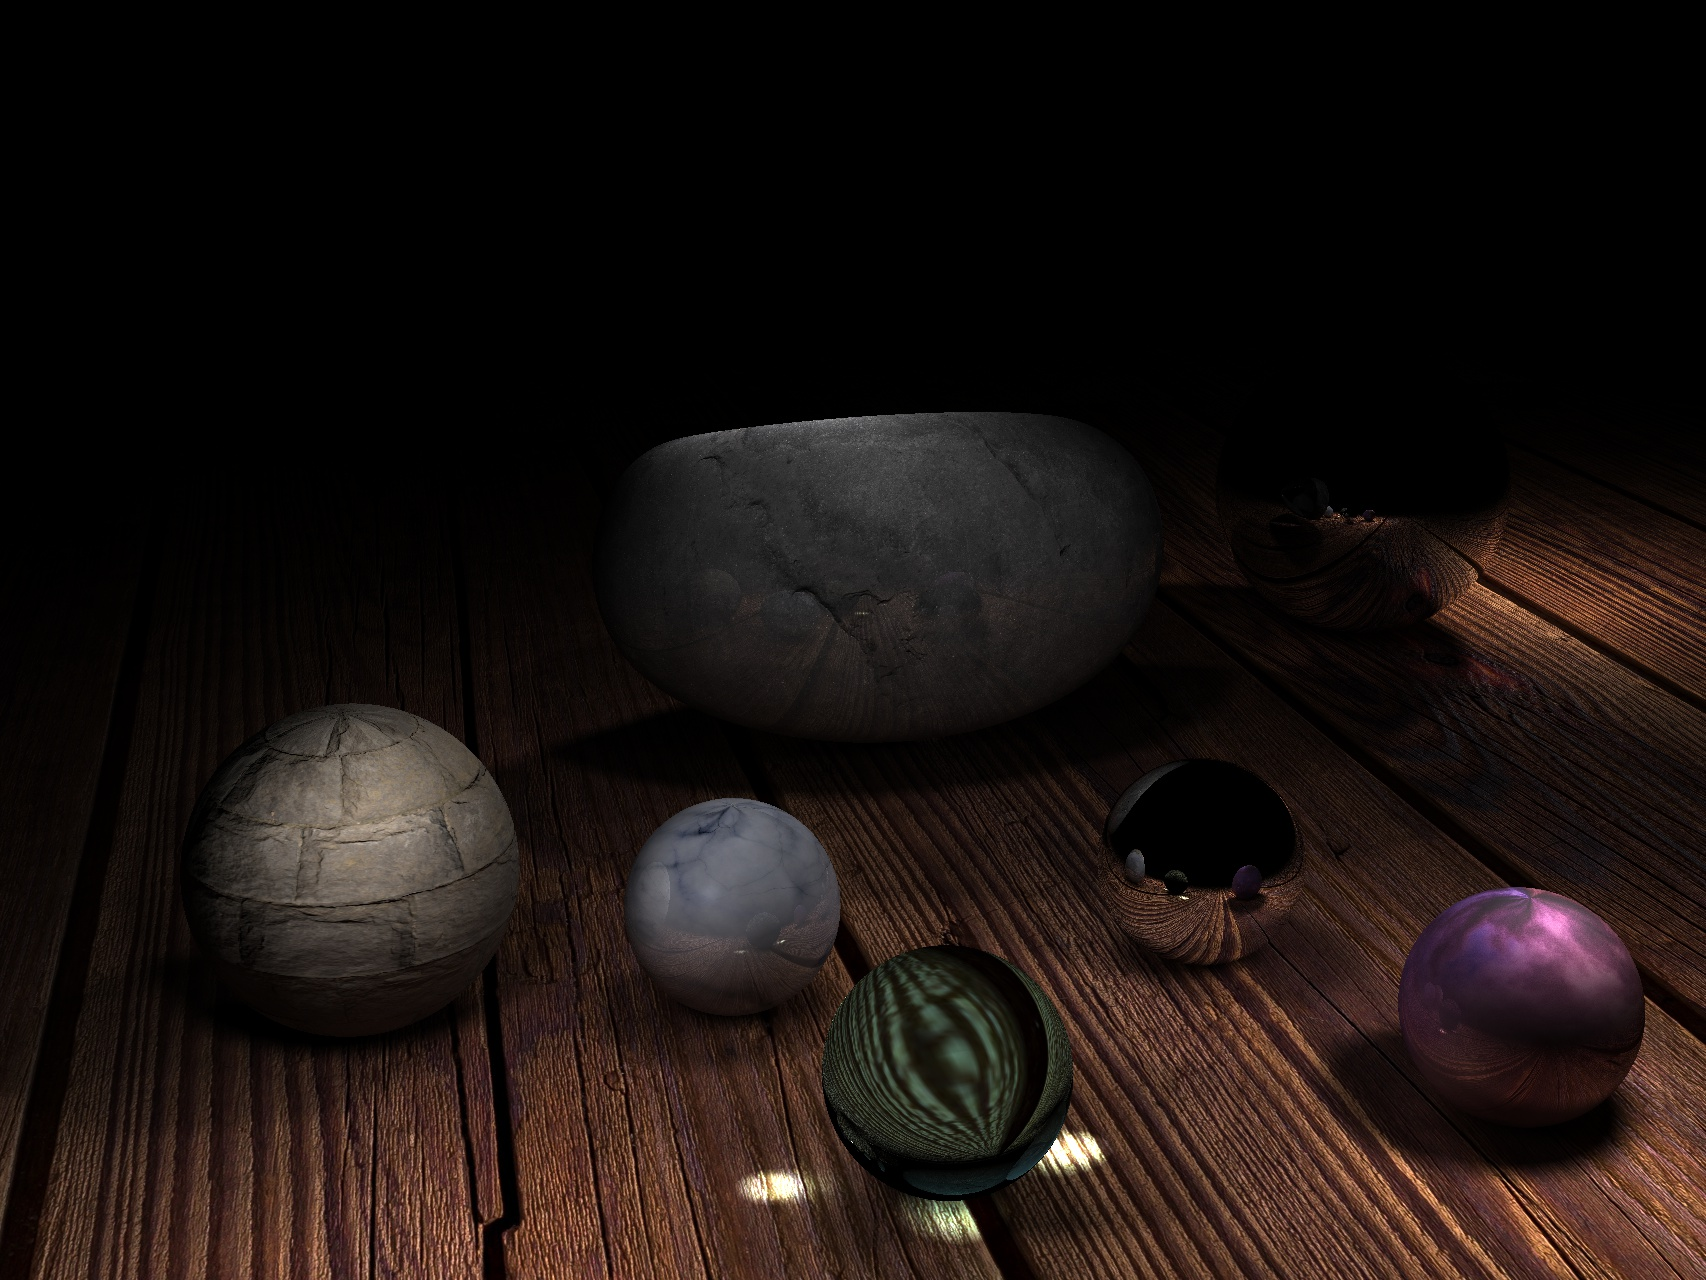
\includegraphics[width=\linewidth]{PPM.jpg}
\caption{最终效果图}
\label{fig:1}
\end{figure}

\begin{figure}[h]
\centering
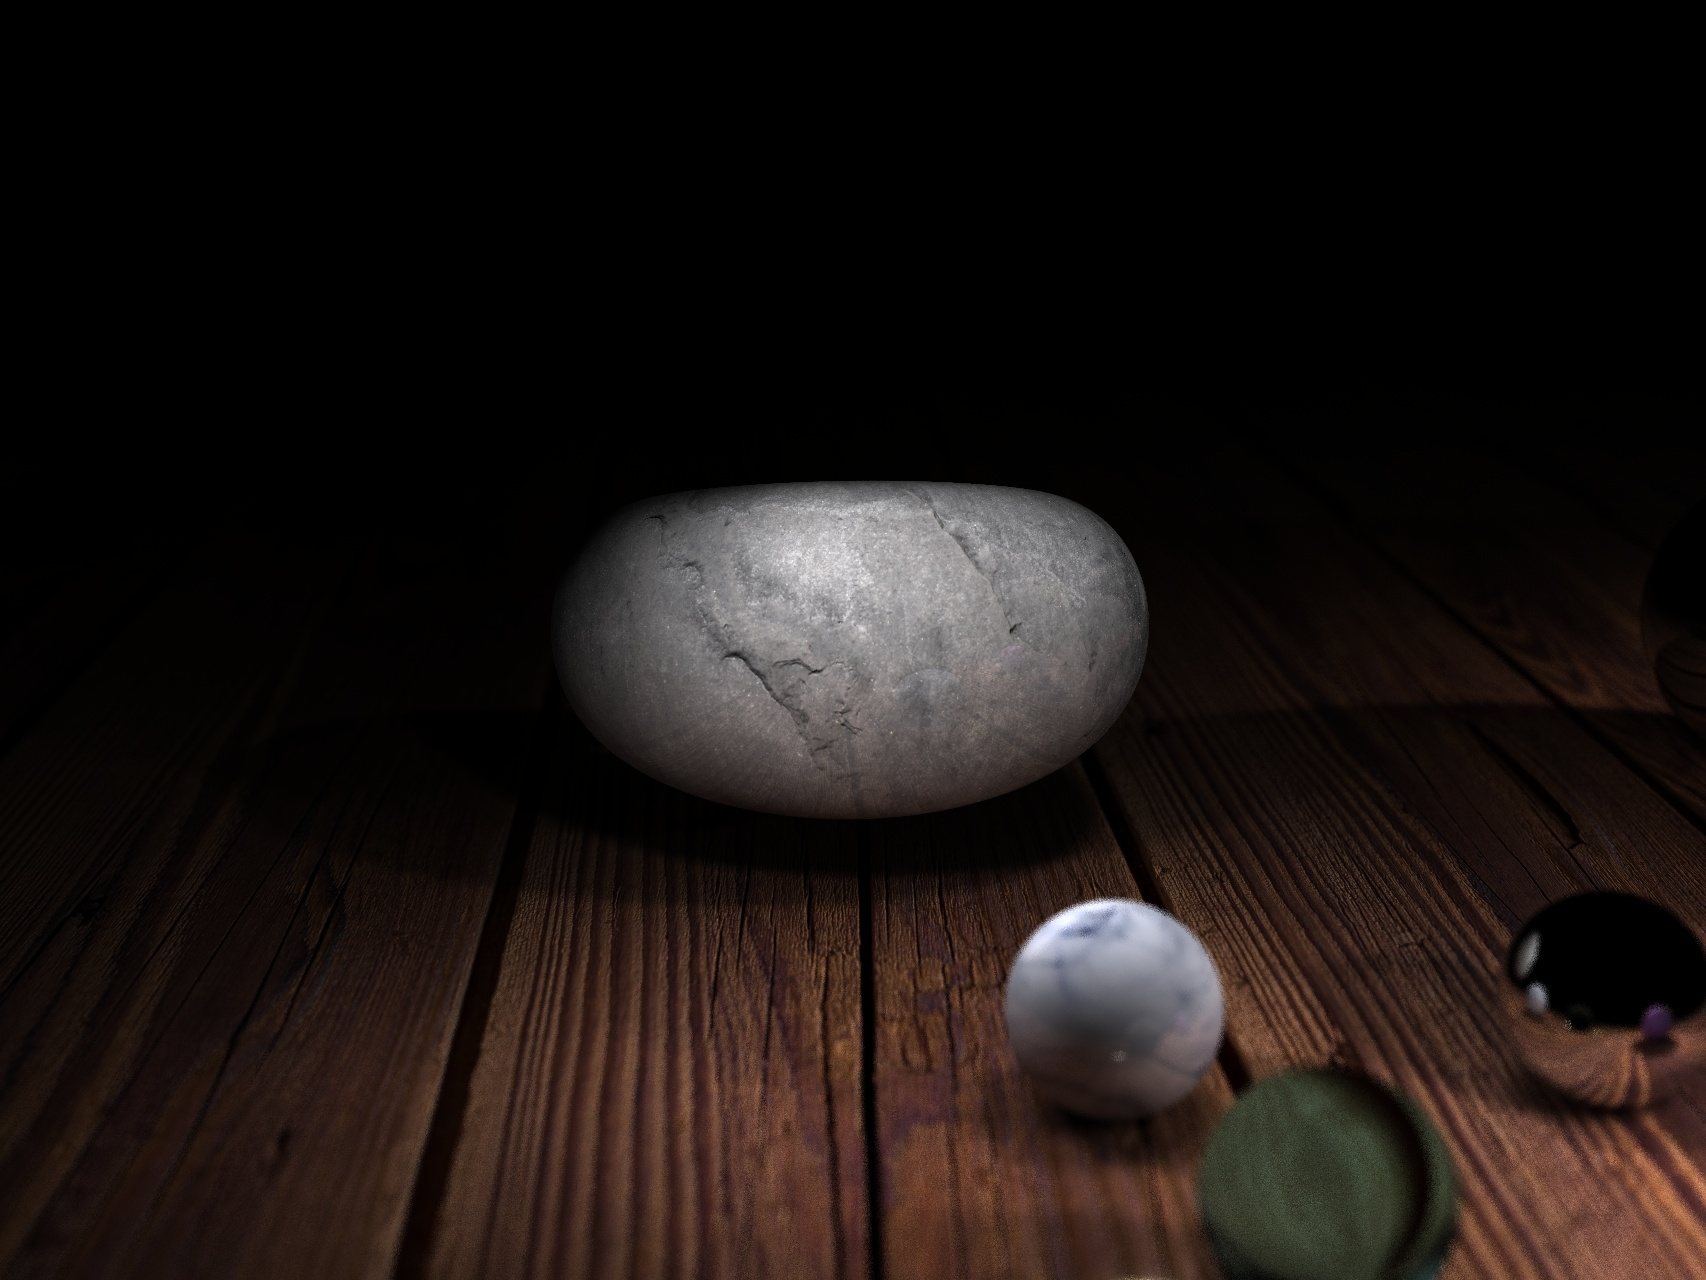
\includegraphics[width=\linewidth]{js.jpg}
\caption{景深效果图}
\label{fig:2}
\end{figure}

\begin{figure}[h]
\centering
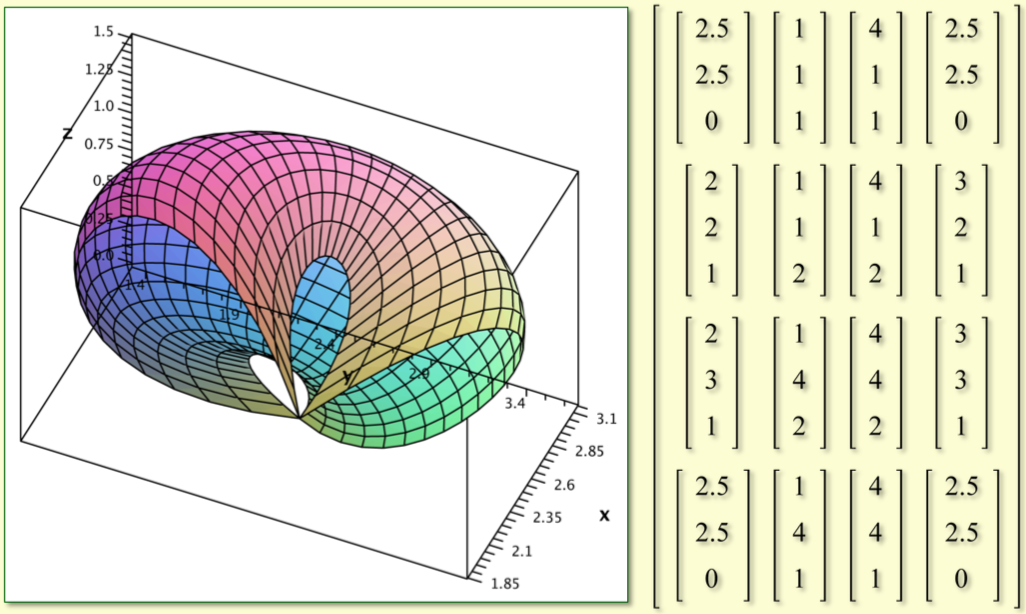
\includegraphics[width=\linewidth]{Bezier.png}
\caption{Bezier曲面控制点及模型}
\label{fig:3}
\end{figure}

\end{document}
